\subsection{Badanie parametrów algorytmu C4.5}
  W implementacji ćwiczenia wykorzystano bibliotekę \textit{rWeka}. Spośród dostępnych
  tutaj parametrów algorytmu C4.5 zostały wybrane i zbadane następujące:

  \begin{table}[H]
    \begin{tabular}{|c|c|p{6cm}|}
      \hline
      \textbf{Nazwa parametru} & \textbf{Wybrane wartości} & \textbf{Opis} \\ \hline
      Reduced error pruning    &  RE = \{ TRUE, FALSE \}   & czy przeprowadzać przycinanie drzewa metodą "reduced error" \\ \hline
      Number of folds for RE pruning & NBF = \{ 2, 10 \}   & liczba podziałów danych (podzbiorów) używanych podczas przycinania "reduced error" \\ \hline
      Min. number of instances per leaf & NBINST = \{1, 10\}& min. liczba instancji w liściu \\ \hline
      Confidence threshold for prunning & CONF = \{0.01, 0.4\}& próg ufności dla przycinania drzewa \\ \hline
    \end{tabular}
    \caption{Zbadane parametry algorytmu C4.5.}
  \end{table}
  Dodatkowo zostało zbadane zachowanie drzewa dla domyślnych wartości parametrów (ustalonych przez autorów biblioteki rWeka).
  Poniższe rysunki obrazują drzewa decyzyjne dla zbioru "Iris" przy zastosowaniu powyższych opcji konfiguracyjnych.

  \subsubsection*{Domyślne opcje konfiguracyjne}
  \begin{figure}[H]
    \center
    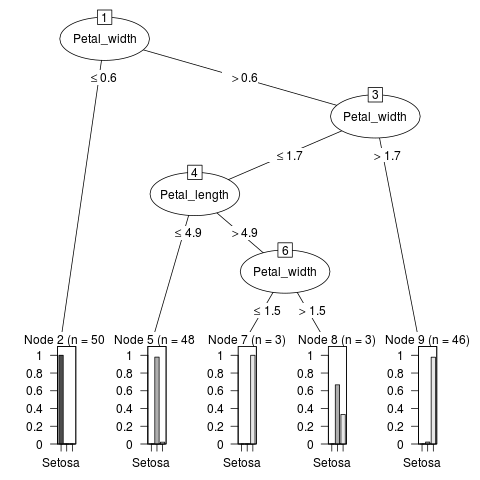
\includegraphics[width=0.4\textwidth]{img/tree_plots/tree_default.png}
    \caption{Drzewo dla domyślnej konfiguracji.}
  \end{figure}

  \subsubsection*{Przycinanie "Reduced error"}
  Zastosowanie przycinania drzewa metodą \textit{reduced error} pozwoliło zmniejszyć głębokość
  otrzymanego drzewo. Dodatkowo można zauważyć, że zastosowanie większej liczby podziałów zbioru 
  danych (foldy) pozwalało zgeneralizować drzewo do 2 reguł. 
  \begin{figure}[H]
    \center
    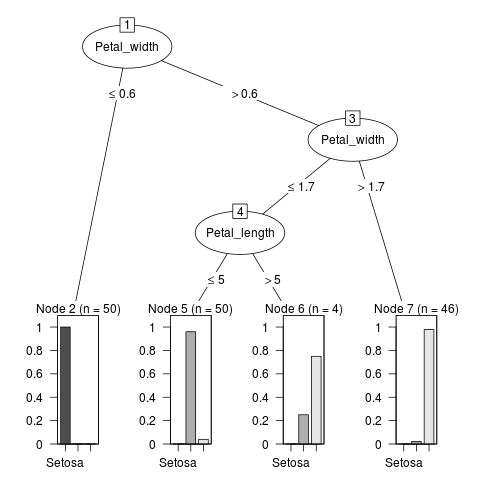
\includegraphics[width=0.5\textwidth]{img/tree_plots/tree_pruned_high_folds.png}
    \caption{Drzewo dla RE = TRUE oraz NBF = 2.}
  \end{figure}

  \begin{figure}[H]
    \center
    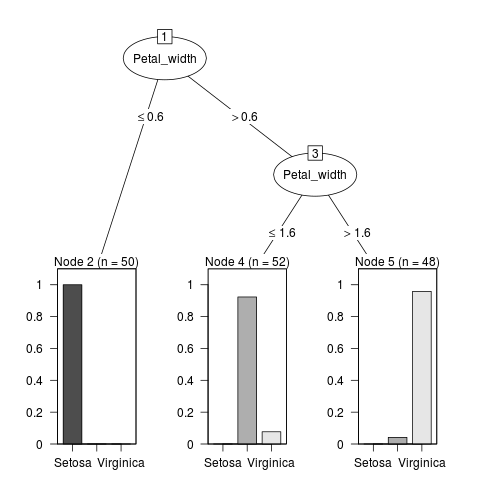
\includegraphics[width=0.5\textwidth]{img/tree_plots/tree_pruned_low_folds.png}
    \caption{Drzewo dla RE = TRUE oraz NBF = 10.}
  \end{figure}

  \pagebreak
  \subsubsection*{Min. liczba instancji w liściu}
  Parametr określający minimalną liczbę instancji w liściu drzewa decyzyjnego znacząco
  wpływa na odporność drzewa na przeuczenie (\textit{overfitting}). W przypadku ustalenia
  tego parametru na wartość równą jeden, ryzyko przeuczenia jest bardzo wysokie, dodatkowo
  można zauważyć, że głębokość drzewa wzrosła (głębokość równa 5) i jest znacznie większa 
  niż w przypadku ustalenia parametru na wartość 10 (głębokość 2).
  \begin{figure}[H]
    \center
    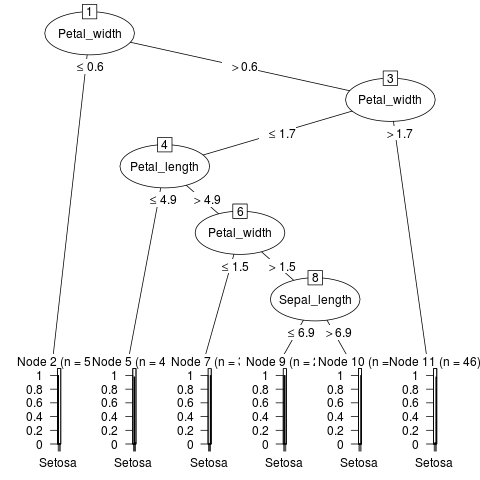
\includegraphics[width=0.5\textwidth]{img/tree_plots/tree_low_leaf.png}
    \caption{Drzewo dla NBINST = 1.}
  \end{figure}

  \begin{figure}[H]
    \center
    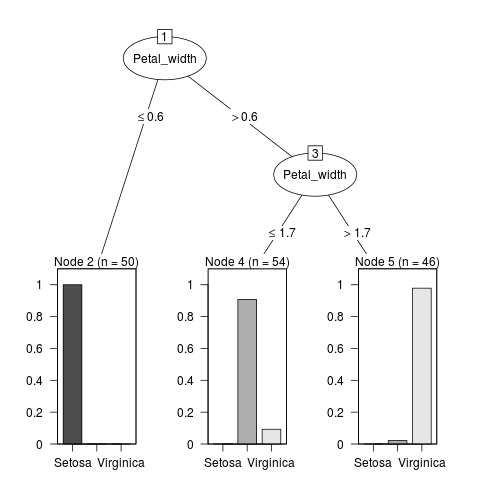
\includegraphics[width=0.5\textwidth]{img/tree_plots/tree_high_leaf.png}
    \caption{Drzewo dla NBINST = 10.}
  \end{figure}
 
  \pagebreak
  \subsubsection*{Próg ufności}
  Zastosowanie wbudowanej metody przycinania (zamiast \textit{reduced error}),
  również pozwoliło ograniczyć głębokość drzewa, jednak efekty nie są tak
  dobre jak w przypadku tamtej metody. Dla parametru progu ufności równego
  0.4 otrzymano drzewo identyczne jak w przypadku zastosowania domyślnych parametrów
  algorytmu. Natomiast zastosowanie bardzo niskiego progu ufności (0.01) pozwalało
  ograniczyć głębokość drzewa o jeden (prawie identyczny z drzewem otrzymanym 
  dla metody \textit{reduced error} z 2 podziałami). 
  \begin{figure}[H]
    \center
    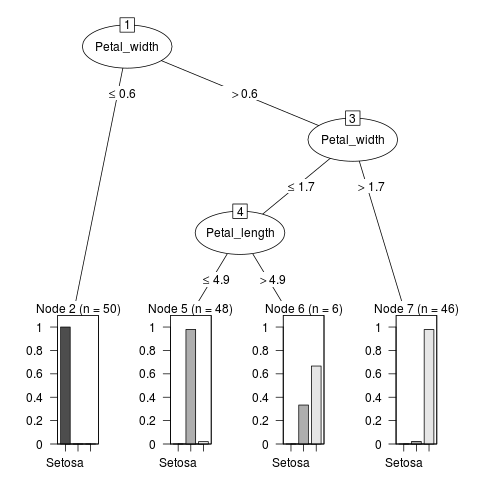
\includegraphics[width=0.5\textwidth]{img/tree_plots/tree_low_conf.png}
    \caption{Drzewo dla CONF = 0.01.}
  \end{figure}

  \begin{figure}[H]
    \center
    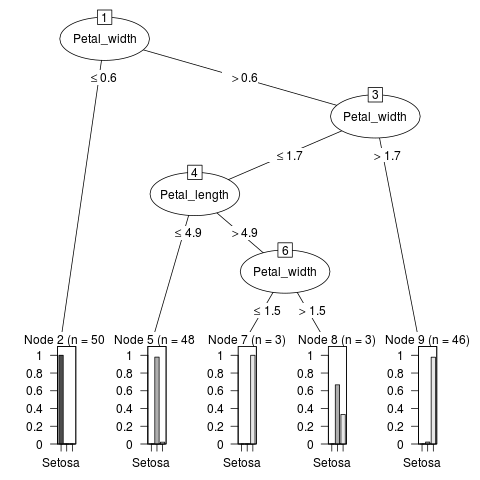
\includegraphics[width=0.5\textwidth]{img/tree_plots/tree_high_conf.png}
    \caption{Drzewo dla CONF = 0.4.}
  \end{figure}
